%--------------------------------------------------------

\begin{frame}
\frametitle{Preliminary Results}

\begin{columns}[T]

%====================================================
% COLUMN 1
%====================================================

\column{0.42\textwidth}

\centering

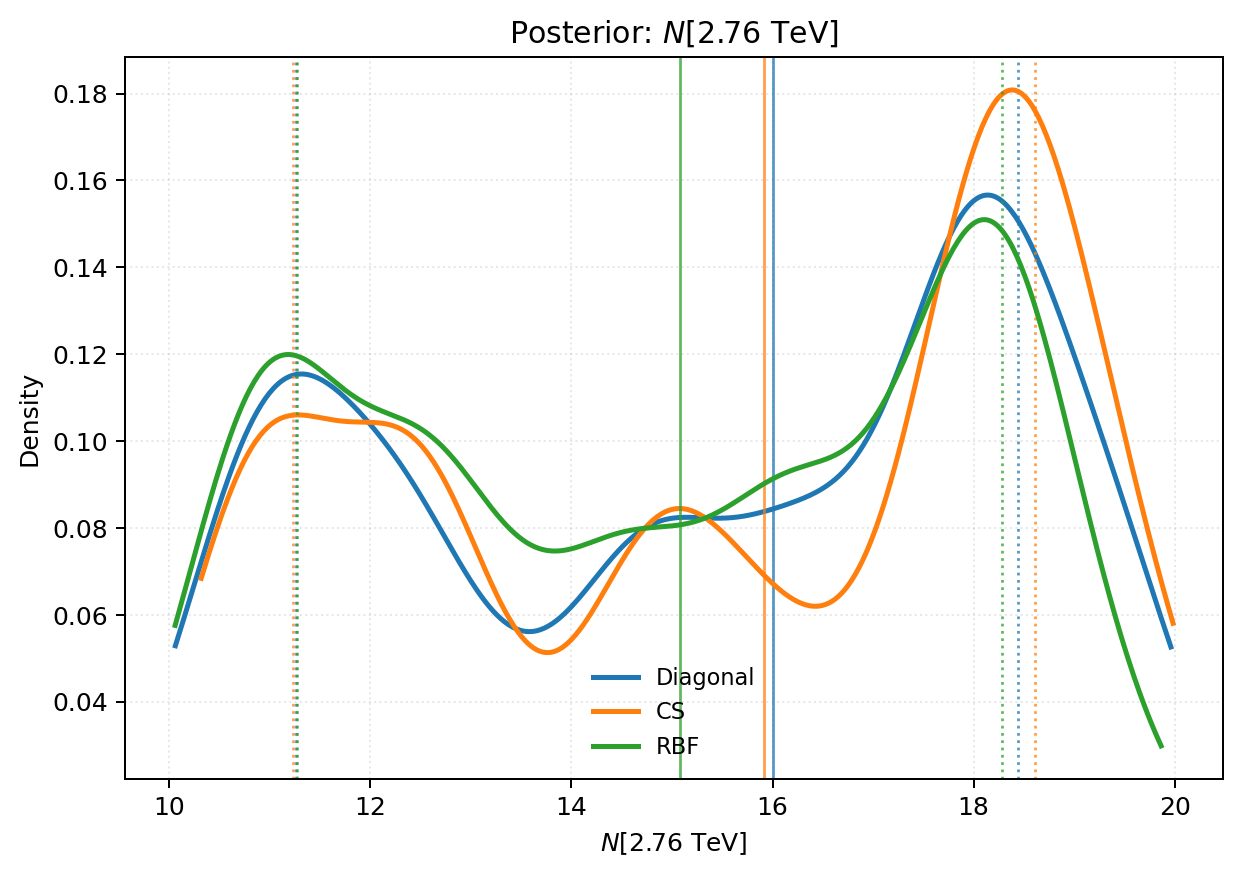
\includegraphics[width=\linewidth]{img/posterior_parameter_01.png}

\vspace{0.18cm}

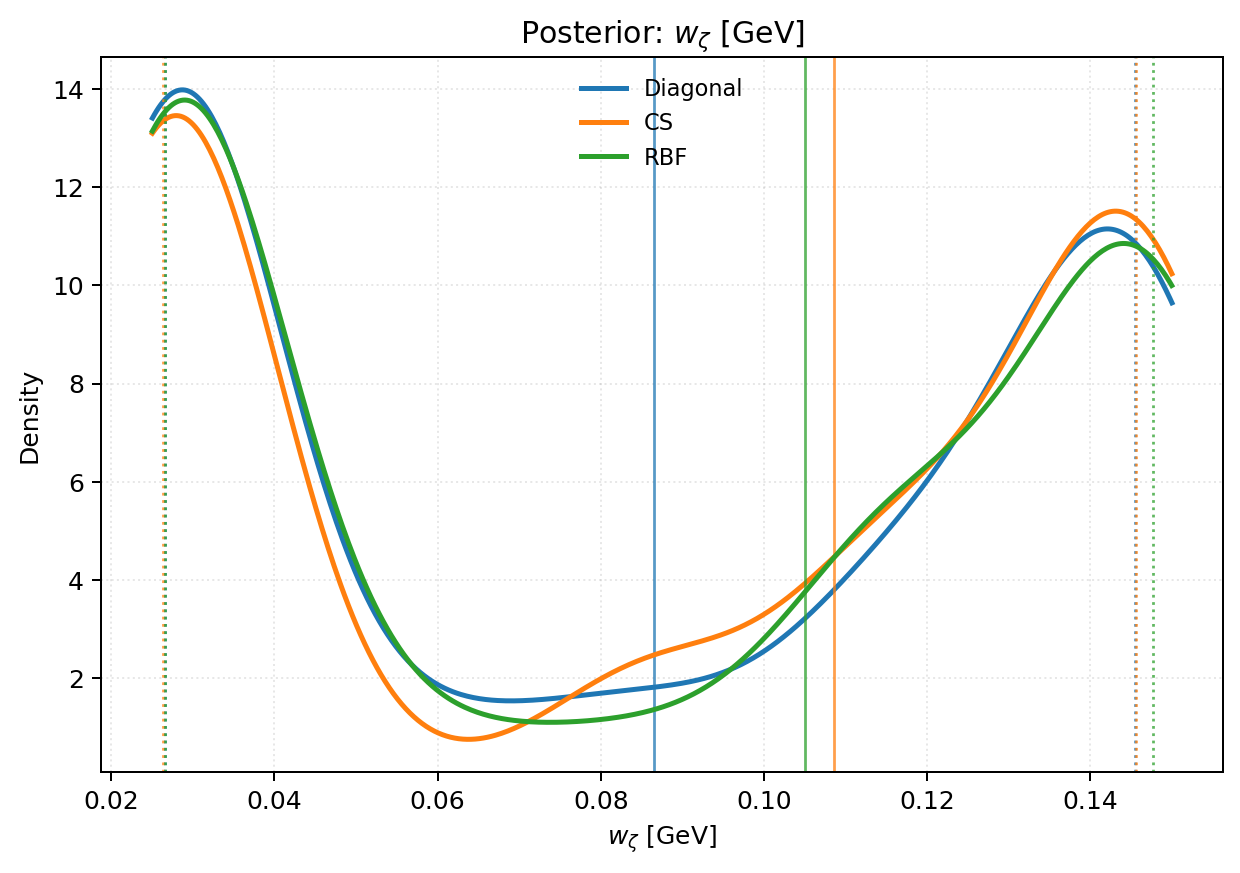
\includegraphics[width=\linewidth]{img/posterior_parameter_14.png}

%====================================================
% COLUMN 2
%====================================================

\column{0.38\textwidth}

\centering

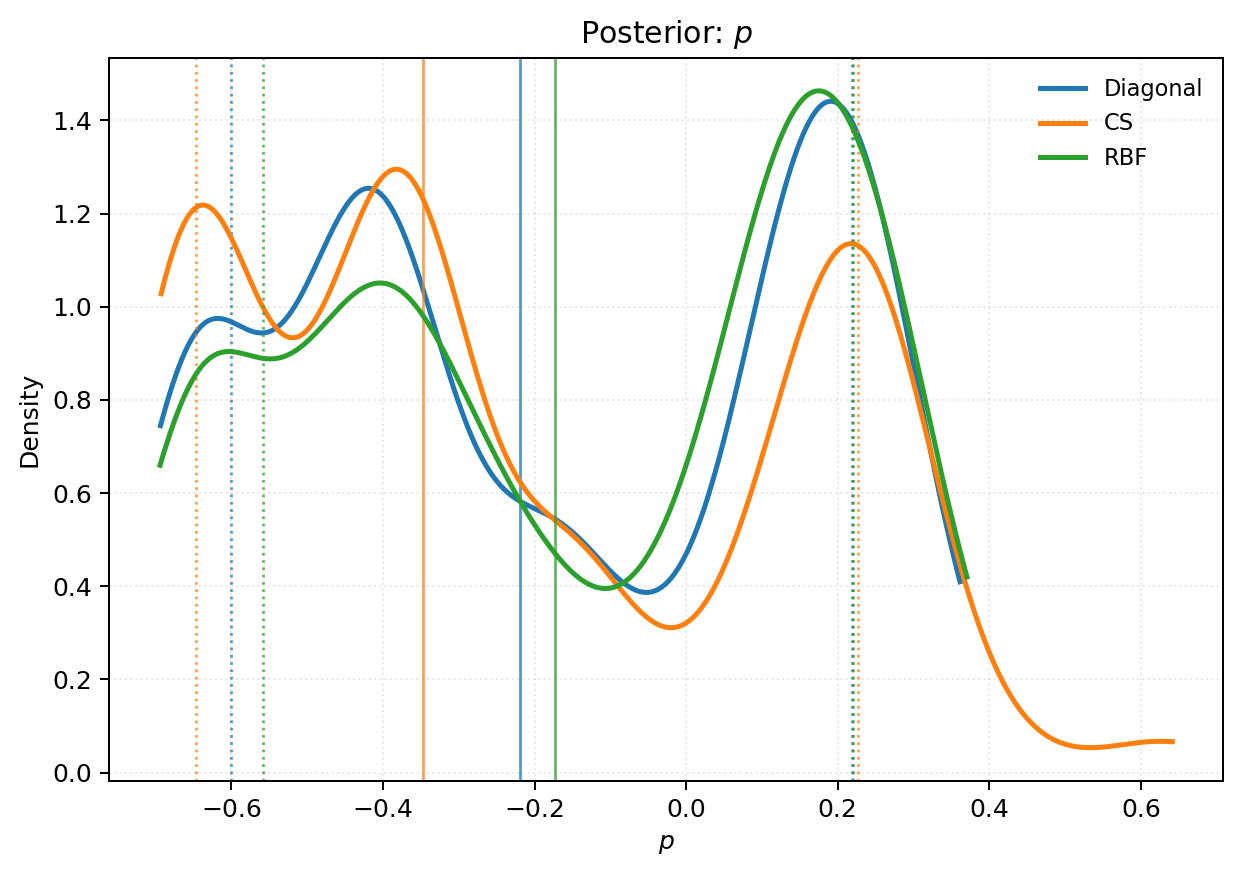
\includegraphics[width=\linewidth]{img/posterior_parameter_02.png}

\vspace{0.72cm}

\scriptsize
\renewcommand{\arraystretch}{1.18}

\begin{tabular}{lr}
\hline
\multicolumn{2}{c}{\textbf{Largest posterior shifts}}\\
\hline
\textbf{Parameter} & \textbf{Max shift}\\
\hline
$p$ & $0.515\sigma$\\
$w_{\zeta}$ & $0.418\sigma$\\
$N$ & $0.307\sigma$\\
\hline
\end{tabular}

\vspace{0.25cm}

\tiny
Largest normalized median shifts among the 17 inferred parameters.

%====================================================
% COLUMN 3
%====================================================

\column{0.20\textwidth}

\centering

% \large
% \textbf{Global comparison }

\vspace{0.68cm}

{\fontsize{11}{12}\selectfont\bfseries
14/17
}

\vspace{0.08cm}

\tiny
parameters with\\
$\Delta<0.3\sigma$

\vspace{0.38cm}

{\fontsize{11}{12}\selectfont\bfseries
3/17
}

\vspace{0.08cm}

\tiny
parameters with\\
$\Delta>0.3\sigma$

\vfill
\vspace{0.24cm}

\tiny
Changing the experimental covariance structure (Diagonal → CS → RBF) produces no statistically significant change in the inferred posterior for the Universal Scaled Spectra calibration, with posterior shifts remaining below $0.6\sigma$ across all inferred parameters.
\end{columns}

\vspace{0.12cm}

\centering
\tiny
Posterior comparison for ALICE Pb--Pb $\sqrt{s_{NN}}=2.76$ TeV, universal spectra calibration.
\end{frame}